\documentclass{ltugproc}

\usepackage[hybrid]{markdown}
\newcommand\term[1]{\textit{#1}}
\newcommand\command[1]{\texttt{#1}}
\newcommand\packagename[1]{\texttt{#1\-.sty}}
\newcommand\option[1]{\texttt{-\/-#1}}
\usepackage{luatexbase}
\usepackage{microtype}
\newcommand\texfourht{\term{\TeX\-4ht}}
\newcommand\texfourhtcmd{\command{tex4ht}}
\newcommand\tfourhtcmd{\command{t4ht}}
\newcommand\makefourht{\command{make4ht}}
% \newcommand\DVI{\acro{DVI}}
\newcommand\extension[1]{\texttt{.#1}}
% make4ht extensions
\newcommand\mkextension[1]{\texttt{#1}}
\newcommand\switch[1]{\texttt{-\/-#1}}



\hyphenation{ma-ke-4-ht tex-4-ht ht-la-tex tex-4-ht-.-sty TeX-4-ht}

\author{Michal Hoftich}
\title{\texfourht: LaTeX to Web publishing}
\address{Charles University, Faculty of Education}
\netaddress{michal.hoftich@pedf.cuni.cz}
\personalURL{https://www.kodymirus.cz}
\begin{document}

\begin{abstract}
  The article gives overview of the current state of development of \texfourht,
  \LaTeX\ to \XML\ conversion system. It introduces \makefourht, a build system for
  \texfourht\ as well as basic ways how to configure \texfourht.
\end{abstract}
\maketitle

\section{Overview of the conversion process}
\texfourht\ is a system for conversion of \TeX\ documents to various output
formats. Most notably \HTML, or \term{OpenDocument Format}, supported by word processors such as Microsoft Word or LibreOffice
Writer. Overview of the system is depicted in the figure \ref{fig:overview}.


The package \packagename{tex4ht} starts the conversion process. The document
preamble is loaded as usual, but it keeps track of all loaded files. 
It loads special configuration files for the
used packages supported by \texfourht\ after the begin of the document.
These configuration with are named as the configured file with a
\extension{4ht} extension.  They can fix clashes between the configured package
and \texfourht, but most notably the package commands can be patched to insert
special marks to the \DVI\ file, so-called
hooks. 

After the package configuration, another type of \extension{4ht} files are loaded.
They populate inserted hooks with tags in the selected output format. In the
last step before processing of the document contents, a \extension{cfg}
provided by the user can configure the hooks with custom tags. Compilation of
the document then continue as usual, resulting in a special \DVI\ file.

The generated \DVI\ file is then processed with the \texfourhtcmd\ command.
This command creates output files, converts various input encoding to UTF-8,
and creates two auxiliary files: \extension{idv} file is a special \DVI\ file that contains
pages to be converted to images. These can be the contents of the \LaTeX\ picture
environment or complex mathematics. The other file with the \extension{lg}
file contains list of output files, CSS instructions, and instructions for
compiling individual pages in the  \extension{idv} file to images.

The last step in the compilation chain is the \tfourhtcmd.
It process the \extension{lg} file and extracts the \acro{CSS} instructions,
converts the images in the \extension{idv} file and can call various external
commands.


\begin{figure*}[hbt!]
  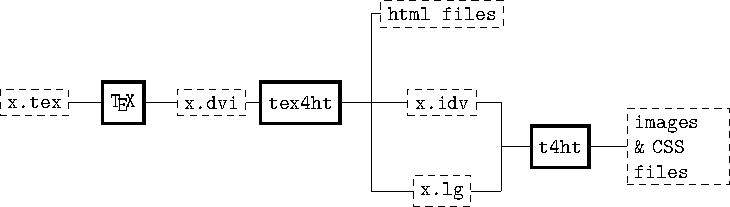
\includegraphics[width=\textwidth]{img/tex4ht_process.pdf}
\caption{\texfourht\ process overview}
\label{fig:overview}
\end{figure*}

\section{Supporting scripts}

Because the entire conversion process consists of several consecutive steps,
we use scripts to make this process easier. The \texfourht\ distribution
contains several of such scripts. They differ in the supported output format, 
\TeX\ engine used, or options passed to the underlying commands.
The most commonly used script  is \command{htlatex}, which uses the \PDF\TeX\ engine with
\LaTeX\ and produces the \HTML\ output. 

Each of the scripts loads the \texfourht\ package without need to specify it in
the document and options from the command line are passed to the package as well to
\texfourhtcmd\ and \tfourhtcmd\ commands.

For example the following command can be used to request the output in the
\acro{XHTML} format in the \acro{UTF-8} encoding:

\begin{verbatim}
htlatex filename.tex \
"xhtml,charset=utf-8"\
"-utf8 -cunihtf"
\end{verbatim}

However, these scripts are inflexible, each time they execute a three-time
compilation of the \TeX\  document. This will ensure the correct structure of
hypertext links and tables, as they require multiple compilations to
function properly. In the following steps, the document is processed by
\texfourhtcmd\ and \tfourhtcmd. 

For example, if the document contains a bibliography or
glossary that are created by external programs, it is necessary to first call
\command{htlatex}, then the desired program, and then \command{htlatex} again.
In the case of larger documents, compilation time in this way may be relatively
long.

The option passing to the underlying commands is also quite difficult.

New build scripts had been created for these reasons. First project that
attempted to simplify the \texfourht\ compilation process was
\command{tex4ebook}. It added support for e-books, in particular in
\term{ePub}, \term{ePub3} and \term{mobi} formats. It added support for use of
command line switches and build files written in the \term{Lua} language.

The main difference between \command{tex4ebook} and \texfourht\ is the third compilation
step. The \tfourhtcmd\ command is used only to create a CSS file. 
Image conversion and execution of the external commands is controlled by the
\command{tex4ebook} itself. In addition, thanks to the build file support, it
is possible to execute commands between individual \TeX\ compilations. For
example, to execute an index processor or \command{bibtex}
after the first compilation.

The library that added the build support provided 
features useful also for other output formats than e-books. It
was extracted as a standalone tool and the \command{make4ht} build system is now a
recommended tool for the \texfourht\ use.


\section{The \command{make4ht} build system}

\makefourht\ enables creation of build scripts in the Lua language. 
It supports execution of arbitrary commands during the conversion,
post-processing of the generated files or setting command for the image
conversion.
Using the so-called modes, it is possible to 
influence the order of compilation using switches directly from the   command
line. For example, the basic script used by \makefourht\ supports the draft mode, which
only runs one compilation of the document instead of the usual three \LaTeX\ compilations. This can
be used to significantly  speed up of the  compilation. 

Currently, only \LaTeX\ is supported, Plain\TeX\ support  is possible, but it is
more complicated and \ConTeXt\ is not supported at all. In the following text we
will focus only on \LaTeX.

\makefourht\ supports a number of switches and options that affect the progress of compiling and processing of the output files.
\makefourht\ can be launched as follows:

\bgroup\small
\begin{verbatim}
make4ht [switches for make4ht] file.tex \
"options for tex4ht.sty" "switches for tex4ht"\
"switches for t4ht" "switches for TeX" 
\end{verbatim}
\egroup


This complicated list is the result  from  the way \command{htlatex} works.
It needs to  pass options for all components involved in
compilation. In most cases, fortunately, there is no need to use all options.
Most of the properties that \texfourhtcmd\ and \tfourhtcmd\ provide can be requested using the
\makefourht\ switches.

\subsection{\makefourht\ command line switches}

All command line switches \makefourht\ supports have a short and long version. In
addition, short switches can be combined together. The following two commands
are identical:


\bgroup\small
\begin{verbatim}
make4ht --lua --utf8 --mode draft filename.tex
make4ht -lum draft filename.tex
\end{verbatim}
\egroup

This command uses Lua\LaTeX\ for the compilation, which will be executed only one
once thanks to the draft mode. The resulting document will be in \acro{UTF-8}
text encoding. The default output format used by \makefourht\ is \HTML5. \command{htlatex} on the other hand uses \HTML4.

In addition to the \switch{lua}, \switch{utf8}, and \switch{mode} switches, there are a number of other useful switches:


\begin{description}
  \item[\switch{config (-c)}] configuration file for \texfourht. Allows user to change tags inserted into output files.
  \item[\switch{build-file (-e)}] select a build file.
  \item[\switch{output-dir (-d)}] the directory where the output files will be copied.
  \item[\switch{shell-escape (-s)}] will use the \texttt{-shell-\/escape} option for \LaTeX, enabling execution of the external commands.
  \item[\switch{xetex (-x)}] the document will be compiled using Xe\LaTeX.
  \item[\switch{format (-f)}] select an output format.
\end{description}

There are other switches, but these are most useful for a common use.


\subsection{Output formats and extensions}

\texfourht\ supports a wide range of \XML-based formats, from \acro{XHTML}, through \acro{ODT} to
\acro{DocBook} and \acro{TEI}. 

The \switch{format} switch supports the following formats: \command{html5}, \command{xhtml}, \command{odt}, \command{tei} and \command{docbook} (it is necessary to use the lowercase letters). 
The default format is \command{html5}. Formats can be selected also using the \packagename{tex4ht} option:

\begin{verbatim}
make4ht filename.tex "docbook"
\end{verbatim}

The advantage of \switch{format} is that it can fix some common issues for the particular formats. 
It can also load extensions. Extensions allow us to influence the compilation
without having to use a build script. The list of extensions to be used can be
written after the format name. They can be  enabled using the plus character,
disabled with the minus character disabled\footnote{Extensions can also be
enabled from the \makefourht\ configuration file, it can be useful to be able
to disable them from  the command line.}. The following command uses the \HTML
Tidy command to fix some common errors in the generated \HTML\ file:


\begin{verbatim}
make4ht -f html5+tidy simple-example.tex
\end{verbatim}

The following extensions are available:

 

\begin{description}
  \item[latexmk\texttt{\_}build] uses the \command{latexmk} build system to compile the document. It will take care of the calling of external commands. For example, it can be used to create a bibliography.

  \item[tidy] cleans the HTML file with the tidy command.

  \item[dvisvgm\texttt{\_}hashes] efficient generation of images using the dvisvgm command. It can use multiple processor cores and only creates images that have been changed or created since the last compilation. This makes the compilation noticeably faster.  

  \item[common\texttt{\_}filters] and \textbf{common\texttt{\_}domfilters}
clean the document using filters. The filters will be discussed later in the  text.

\item[mathjaxnode] convert \MathML\ math code into special \HTML\ using
  \term{MathJax Node Page}\footnote{\url{https://github.com/pkra/mathjax-node-page/}}.
  It produces mathematics that can be viewed in web browsers without the 
  \MathML\ support. The rendering of the result doesn't need JavaScript, which results in much faster display of the document compared  to the regular MathJax.

\item[staticsite] creates a document that can be used for static page generators such as \term{Jekyll}\footnote{\url{https://jekyllrb.com/}}. These are useful for creating a blog or similar more complex website.
\end{description}


\subsection{Configuration file for make4ht}

\makefourht\ supports build scripts in the  Lua language. They can be used to
call external commands, to pass parameters to an executed command, to apply filters to
the output files, to affect the image conversion, or to configure extensions.

The \extension{make4ht} configuration file is a special build script that is loaded
automatically and should contain only general configurations shared between documents. In contrast,
normal build files may contain configurations useful only for the current document. The
configuration file can be located in the  directory of the current   document or in  its
parent directories. 

This can be useful, for example, for maintaining a blog.
Each document is located in its own directory. In the parent directory
can be located a configuration file to ensure proper processing. Here's a small
example: 

\begin{verbatim}
filter_settings "staticsite" {
  site_root = "output" 
}

Make:enable_extension("common_domfilters")
if mode=="publish" then
  Make:enable_extension("staticsite")
  Make:htlatex {}
end

\end{verbatim}

This configuration file sets the option \verb|site_root| for the
\mkextension{staticsite} extension using the \texttt{fil\-ter\-\_\-set\-tings}
command.  This command can be used to set options for filters but also for
extensions.
The name of the filter or extension is separated from the command by a space,
followed by another space-separated field, where options can be set.

Another used command is \texttt{Make:\-enable\-\_\-ex\-ten\-sion}, which enables the
extension. In this case the \verb|common_domfilters| extension is used in every
compilation, but the \mkextension{staticsite} extension is used only in the  \term{publish}
mode. In this mode it is also necessary to use the \verb|Make:htlatex{}| to
require at least one \LaTeX\ compilation.

Now it is possible to run \makefourht\ in the publish mode:


\begin{verbatim}
make4ht -um publish simple-example.tex
\end{verbatim}

The \texttt{output} directory will be created if it does not already exist. \HTML\ and \CSS\ files will be copied here. The static site generator must be configured to look up for files here and it needs to be executed manually, the extension doesn't do that. 

The resulting HTML file may take the following form: 


\begin{verbatim}
---
time: 1544811015
date: '2018-12-14 18:10:47'
title: 'sample'
styles:
- '2018-12-14-simple-example.css'
meta:
- charset: 'utf-8'
---
<p>Sample document</p>
\end{verbatim}

The document header enclosed between the two \verb|---| contains variables in the \acro{YAML}
format extracted from the \HTML\ file. Only the contents of the document body
remains in the document, old header is stripped off. The
static generator can then create a page based on the template and the variables
in the \acro{YAML}  header.

This was just a basic example, filters and extensions have much wider configurable options, all of which are described in the \makefourht\  documentation\footnote{\url{https://ctan.org/pkg/make4ht}}.


\subsection{Build files}

In the compilation scripts it is possible to use the same procedures as in   the configuration
file, but more focused on the particular compiled document. 
The following code shows use of the DOM filters. These take advantage of the
\term{LuaXML}\footnote{\url{https://ctan.org/pkg/luaxml}} library. It allows to process XML files
using the Document Object Model (DOM) interface. This makes it easy to
navigate, edit, create or delete elements.

The use of DOM filters is shown on the following example for Lua\LaTeX:


\begin{verbatim}
\documentclass{article}
\begin{document}
Test {\itshape háčků}
\end{document}
\end{verbatim}


Because of the known error in processing the \DVI\ file with the \texfourhtcmd\ command, 
each accented character 
in the generated \HTML\ file 
will be placed in  a separate \verb|<span>| element:


\begin{verbatim}
<!--l. 4--><p class="noindent" >Test 
<span class="rm-lmri-10">h</span><span 
class="rm-lmri-10">á</span><span 
class="rm-lmri-10">čk</span><span 
class="rm-lmri-10">ů</span> </p> 
\end{verbatim}

The following build file removes this by using the built-in \mkextension{joincharacters} DOM
filter. In addition, it changes the value of class attribute for all \verb|<p>| elements to
\term{mypar}, just to show how to work with the  DOM Interface:

\begin{verbatim}
local domfilter = 
  require("make4ht-domfilter")

local function domsample(dom)
  -- the following code will process
  -- all <p> elements
  for _, par in 
    ipairs(dom:query_selector("p")) do
    -- set the "class" attribute
    par:set_attribute("class", "mypar")
  end
  return dom
end

local process = domfilter({
  "joincharacters", 
  domsample
})
Make:match("html$", process)
\end{verbatim}

The script uses the standard Lua \texttt{require} function to  load the
\texttt{make4ht-domfilter} library. This creates a \texttt{domfilter} function that takes a list
of DOM filters to execute as a parameter. 

Each call to the \texttt{domfilter} function
creates another function with a chain of filters specified in a table. 
Parameters in the   fields can be either the name of an existing DOM
filter, or a function defined in the file. 

The filter chain can be then used in the \texttt{Make\-:\-ma\-tch}
function. It takes a filename pattern to match files for which the filters
should be executed, and the filter chain.


The \texttt{process} function will run
on each file whose filename ends with \texttt{html} in this case.

The resulting \HTML\ file does not contain the extra \verb|<span>| elements and the \verb|<p>| element has a class attribute value of \texttt{mypar}:

\begin{verbatim}
<!-- l. 3 --><p class='mypar'>
Test <span class='rm-lmri-10'>háčků</span> 
</p> 
\end{verbatim}

More complex build file with external commands execution or configuration of the image generation may look as follows:

\begin{verbatim}
Make:add("biber", "biber ${input}")
Make:htlatex {}
Make:biber {}
Make:htlatex {}
Make:image("png$")
"dvipng -bg Transparent -T tight "..
-o ${output} "-pp ${page} ${source}")
Make:match("html$")
"tidy -m -utf8 -asxhtml -q -i ${filename}")
\end{verbatim}


The \verb|make:add| command may be used to add a new command, like
\texttt{biber} in this case. The second parameter is a formatting string, which
may contain \verb|${variable name}| templates, which are replaced by parameters
set by \makefourht. The \verb|${input}| will be replaced with the input file name for example.

The added command can be then used using the \verb|Make:command name {}|
command. Additional variables may be set in the table passed as the argument.

The \texttt{Make:htlatex} command is built-in and requires one execution of \LaTeX\ with active \texfourht.

The \texttt{Make:image} command configures the image conversion. Three
variables are available, \texttt{page} contains the page number of the image in
the \DVI\ file, \texttt{output} is the name of the output image, and \texttt{source} is
the name of the \extension{idv} file.

The use of the \texttt{Make:match} command had been shown in the previous
example, but it may also contain string with the command to be executed. The
\texttt{filename} variable contains filename of the currently processed
generated file.




\section{\texfourht\ configuration}


Output format tags embedded in a document are fully configurable using several
mechanisms. The easiest way to use the \packagename{tex4ht} package options, more advanced choice is
to use a custom configuration file and the most powerful  option is to use the  \extension{4ht} files.

When a \TeX\ file is compiled using \makefourht\ or another compilation script, the
\packagename{tex4ht} package is loaded before the document itself. Package
options are obtained from the  compilation script arguments. As a result, it is not necessary
to insert the \packagename{tex4ht} package in the  document itself.

The file loading mechanism is modified to register each loaded file with
\texfourht. For some packages, \texfourht\ also contains code that prevents it from
loading, or to immediately override some macros. This is necessary for packages
that are incompatible with   \texfourht, such as \texttt{Fontspec}.

After execution of  the document preamble, the configuration files for the packages
detected during processing are loaded. These files are named as a filename of the configured package
without the extension plus the  \extension{4ht} extension. Their main function is to insert configurable
macros, called hooks, into the commands provided by the package. In general, it
is better not to redefine macros, only to patch them with the commands
\texfourht\ provides for this purpose is enough in most cases.

Output format configuration files are loaded after the package configuration
files are processed. These define the contents of configuration macros, or hooks as we call them.
Not only the output format tags are inserted here, they can contain
any valid \TeX\ commands. 

\subsection{\packagename{tex4ht} options}

Many configurations are conditional, they are executed only in the presence of some options 
for \packagename{tex4ht} package.
Each output format configuration file can test any option, which means that there is no final list of possible options and 
each output format can support different set of options.

Because it is not recommended to put the \texttt{tex\-4ht\-.sty} package directly into the document, it is possible to pass the options in other ways. 
The easiest way is to use the compilation script argument. It is always the argument following the document name:

\begin{verbatim}
make4ht filename.tex "mathml,mathjax"
\end{verbatim}

Two options used in this example are \texttt{mathml} and \texttt{mathjax}. 

Another possibility to  pass options is to use the \cs{Preamble}  command in the private configuration file. We'll show it in the  next section.

As already mentioned, there is no final list of options, each output format can support any number of them.

However, we can show some choices regarding mathematical outputs in  \HTML.
Normal configuration for mathematical environments produces a blend of rich
text and images for more complex outputs, if that cannot be easily created with
HTML elements. Often this output doesn't look good. As an alternative,
it is possible to use images for all math content. This can be achieved by using the \texttt{pic-m}
options for inline mathematics and \texttt{pic-\meta{environment name}} for mathematical
environments. For example, the  \texttt{pic-align} option will require pictures for all \texttt{align} environments.

By default, images are created in the \acro{PNG} format. Higher quality can be
achieved using the \acro{SVG} vector format. This can be enforced using the
\texttt{svg} option.

\texfourht\ documentation is quite spartan. More comprehensive information
about the available configurations can be found in the  \extension{log} file after the compilation 
of a document using the \texttt{info} option.

Options listed  in the example above, \texttt{mathml} and \texttt{mathjax},
provide the best mathematical content output in. The \MathML\ markup language, requested by the first option,
encodes the mathematical information, but its support in Web browsers
is poor. The second option requests the \term{MathJax} library, which can render the \MathML\ output in all
browsers with the  JavaScript support.

\texttt{mathjax} option used without \texttt{mathml} completely turns off
compilation of math, all math content remains in the \HTML\ document as raw
\LaTeX\ macros. \term{MathJax} then processes the document and renders the math in the
correct way. The disadvantage of this method is that \term{MathJax} does not support
all packages and user commands, it needs a special configuration in these
cases. Sometimes it is not even possible to emulate more complex macros.




\subsection{Private configuration file}

The private configuration file can be used to insert custom content into the configuration hooks. This file has a special structure:

\begin{verbatim}
... Preamble definitions
\Preamble{tex4ht.sty options}
... Normal configurations...
\begin{document}
... Configurations for HTML head
\EndPreamble
\end{verbatim}

The following commands must be always included in the configuration file: \verb|\Preamble|, \cs{begin}\-\tubbraced{document} and \verb|\EndPreamble|. 
The configuration file name can be pass to \makefourht\ using the \switch{config} (or \texttt{-c}).

\begin{verbatim}
make4ht -c myconfig.cfg filename.tex
\end{verbatim}

The full file path must be used if the configuration file is not placed in the current working directory.

Several configuration commands exist. The most important are
\verb|\Configure| for common configurations, 
\verb|\ConfigureEnv| for configuration of \LaTeX\ environments,
or \verb|\ConfigureList| for the configuration of the list environments.

The \verb|\HCode| command is used for insertion of the output format tags.
The \verb|\Hnewline| command inserts a newline in the output document.
\verb|\Css| can be used to insert a content to the \acro{CSS} file.


The following example configures the hooks for the \cs{textit} command to insert the \verb|<em>| element.

\begin{verbatim}
\Configure{textit}{\HCode{<em>}\NoFonts}
{\EndNoFonts\HCode{</em>}}
\end{verbatim}

The \cs{Configure} supports a variable number of arguments. It depends on the
hooks definition hooks, how many arguments are needed. The first argument is
always the name of the configuration, the other arguments then put the code in
the hooks. Typically, configuration requires two hooks -- one places the
code before the start of the command, the second behind it. That's the case of 
the configuration for \texttt{textit} used above. The configuration name may
match the name of the configured command, but it is not always the case. 
The package \extension{4ht} file may choose the configuration names arbitrary.

The \cs{NoFonts} command disables inserting formatting elements for fonts when processing a \DVI
file. \texfourht\ automatically creates basic formatting for used fonts. This
makes it possible to create a document with basic formatting even for unsupported commands.
It is not desirable when the command is configured using custom \HTML\ elements.

Paragraph handling is a complicated issue. \texfourht\ sometimes put paragraph
tags in inappropriate
places. This applies primarily to environment configurations that can contain
several paragraphs and place their entire content in one element. It may happen
that the starting paragraph mark is placed before the beginning of this
element, but it should be placed right after that. The \cs{IgnorePar} command can prevent 
the insertion of a tag for the next paragraph. \cs{EndP} inserts
a closing tag for the previous paragraph. There are more commands to work with
paragraph, but these are the most important.

To illustrate this issue, 
the following example uses the hypothetical \texttt{rightaligned} environment to be placed in  an \verb|<article>| element.


\begin{verbatim}
\ConfigureEnv{rightaligned}
{\HCode{<section class="right">}}
{\HCode{</section>}}{}{}
\end{verbatim}

The \cs{ConfigureEnv} expects five parameters. The first one should contain the configured
environment name. Contents of the second parameter are inserted at the beginning of the
environment, the third parameter contents are added at the end of the environment. The other two parameters
are used only if the configured environment is based on a list. In most cases
they may be left blank. The \HTML\ code created by the configuration in the previous listings can look
like in the following way:


\begin{verbatim}
<p class="indent" ><section class="right">
...
</p><p class="indent></section>
\end{verbatim}

This code is invalid. The terminating tag for the \verb|<p>| element is placed
at the wrong nesting level. Invalid code can cause the DOM filters and other post-processing tools expecting well-formed \XML\ file to 
fail. This situation must be avoided.

The correct configuration is somewhat more complicated: 

\begin{verbatim}
\ConfigureEnv{rightaligned}
{\ifvmode\IgnorePar\fi\EndP
\HCode{<section class="right">}\par}
{\ifvmode\IgnorePar\fi\EndP
\HCode{</section>}}
{}{}
\end{verbatim}

In this case the insertion of tags for paragraphs is controlled, which results  is in a correct structure:

\begin{verbatim}
<section class="right">
<!--l. 9--><p class="indent" >
...
</p></section>
\end{verbatim}

It is also possible to request the conversion of part of a document to an image. 
This can be requested using commands \cs{Picture*} or \cs{Picture+} respectively. 
The difference between them is that the first one processes its content as a vertical box. 
The content between these any of these commands and closing \cs{EndPicture} is converted to an
image.


The following example creates an image for the text contained in the \texttt{topicture} environment : 

\begin{verbatim}
\documentclass{article}
\newenvironment{topicture}
{\bfseries}{}
\begin{document}
\begin{topicture}
Contents of this environment 
will be converted as an image.
\end{topicture}
\end{document}
\end{verbatim}

The configuration for the \texttt{topicture} environment uses the \cs{Picture*}:

\begin{verbatim}
\ConfigureEnv{topicture}{\Picture*{}}
{\EndPicture}{}{}
\end{verbatim}

Resulting document will contain image with text contained in the \texttt{topicture}
environment as was typeset in the \DVI\ file.



\section{Conclusion}

The \texfourht\ configuration options are extensive.  We touched only the
basics in the previous text. It, however, should be enough to solve the 
basic issues that the users of this system face. 
We skipped examples of how to add configurations for a  new \LaTeX\ package. This topics will be hopefully addressed in a future.

The system is easier and more efficient to use than in the past, thanks to the \makefourht\ build system.

The new documentation for \texfourht\ is being developed with financial support by \acro{CSTUG}. It will describe the most useful user configurations, as well as technical details of the system.




\end{document}
